\documentclass[12pt]{article}
\usepackage[spanish]{babel}
\usepackage{natbib}
\usepackage{url}
\usepackage[utf8x]{inputenc}
\usepackage{amsmath}
\usepackage{float}
\usepackage{subfig}
\usepackage{graphicx}
\graphicspath{{images/}}
\usepackage{parskip}
\usepackage{fancyhdr}
\usepackage{vmargin}
\setmarginsrb{3 cm}{2.5 cm}{3 cm}{2.5 cm}{1 cm}{1.5 cm}{1 cm}{1.5 cm}

\title{\#3 Interpolación}							% Título
\author{Alejandro Guirado García}											% Autores
\date{\today} %Aquí pueden cambiarla%					% Fecha de edición

\makeatletter
\let\thetitle\@title
\let\theauthor\@author
\let\thedate\@date										
\makeatother

\pagestyle{fancy}
\fancyhf{} %Si quieres ponerle otro encabezado/pie de pagina%
\lhead{\thetitle}
\cfoot{\thepage}

\begin{document}

%%%%%%%%%%%%%%%%%%%%%%%%%%%%%%%%%%%%%%%%%%%%%%%%%%%%%%%%%%%%%%%%%%%%%%%%%%%%%%%%%%%%%%%%%

\begin{titlepage}
	\centering
    \vspace*{0.5 cm}
    \includegraphics[scale = 0.5]{logo}\\[0.5 cm]	% University Logo
    \textsc{\Large Universidad de Sonora}\\[1.0 cm]	% University Name
	\textsc{\Large División de Ciencias Exactas y Naturales}\\[0.5 cm]				% Course Code
	\textsc{\large Física Computacional I}\\[0.5 cm]				% Course Name
	\rule{\linewidth}{0.2 mm} \\[0.4 cm]
	{ \huge \bfseries \thetitle}\\
	\rule{\linewidth}{0.2 mm} \\[0.5 cm]
 
	
	\begin{minipage}{\textwidth}
		\begin{flushleft} 
			\emph{\Large Integrante:} \large \\
			\theauthor
			\end{flushleft}
	\end{minipage}\\[1 cm]
	{\large \thedate}\\[2 cm]
 
	\vfill
	
\end{titlepage}

%%%%%%%%%%%%%%%%%%%%%%%%%%%%%%%%%%%%%%%%%%%%%%%%%%%%%%%%%%%%%%%%%%%%%%%%%%%%%%%%%%%%%%%%%

\section{Introducción}

En está prácica interpolaremos puntos aleatorias con la función para interpolar de python.  Primeramente se explicará en que consiste interpolar; En el subcampo matemático del análisis numérico, se denomina interpolación a la obtención de nuevos puntos partiendo del conocimiento de un conjunto discreto de puntos.

En ingeniería y algunas ciencias es frecuente disponer de un cierto número de puntos obtenidos por muestreo o a partir de un experimento y pretender construir una función que los ajuste.

Otro problema estrechamente ligado con el de la interpolación es la aproximación de una función complicada por una más simple. Si tenemos una función cuyo cálculo resulta costoso, podemos partir de un cierto número de sus valores e interpolar dichos datos construyendo una función más simple. En general, por supuesto, no obtendremos los mismos valores evaluando la función obtenida que si evaluamos la función original, si bien dependiendo de las características del problema y del método de interpolación usado la ganancia en eficiencia puede compensar el error cometido.

En todo caso, se trata de encontrar una función que:
\begin{equation}
f(x_k)=y_k, k=1,...,n
\end{equation}
  
  Fue proporcionado un código base para modificar el cual es el siguiente: 
  
  
  \begin{verbatim}
import numpy as np
import matplotlib.pyplot as plt
from scipy.interpolate import interp1d

# Original "data set" --- 21 random numbers between 0 and 1.
x0 = np.linspace(-1,1,21)
y0 = np.random.random(21)

plt.plot(x0, y0, 'o', label='Data')

# Array with points in between those of the data set for interpolation.
x = np.linspace(-1,1,101)

# Available options for interp1d
options = ('linear', 'nearest', 'zero', 'slinear', 'quadratic', 'cubic', 10)

for o in options:
    f = interp1d(x0, y0, kind=o)    # interpolation function
    plt.plot(x, f(x), label=o)      # plot of interpolated data

plt.legend()
plt.show()
\end{verbatim}
 Este código nos proporcionó la siguiente interpolación:
 \begin{figure}[H]
\centering
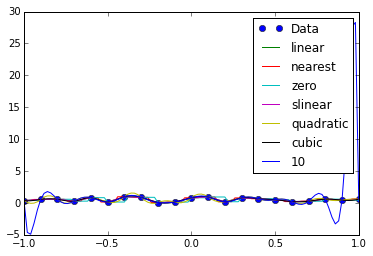
\includegraphics[height=5cm]{index.png}
\end{figure}
\begin{enumerate}


\section{Interpolaciones}
\item La primera interpolación es dados 10 puntos aleatorios entre x=0 y x=3, para f(x)=sin(2x).

\begin{verbatim}
import numpy as np
import matplotlib.pyplot as plt
from scipy.interpolate import interp1d


x0 = np.random.random(10)
x = x0*3
y = np.sin(2*x)

plt.plot(x, y, 'o', label='Data')

xp = np.linspace(min(x), max(x), 51051)
                
  options = ('linear', 'quadratic', 'cubic')
for o in options:
    f = interp1d(x, y, kind=o)    
    plt.plot(xp, f(xp), label=o)    
    
plt.legend([ 'linear', 'quadratic', 'cubic'], loc='best')
plt.show()
\end{verbatim}
 Este código nos proporcionó la siguiente interpolación:
 \begin{figure}[H]
\centering
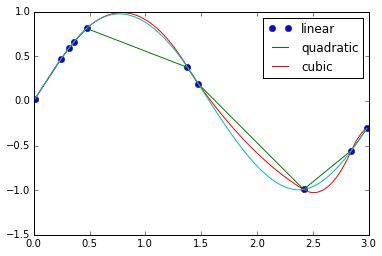
\includegraphics[height=5cm]{sin.png}
\end{figure}


\item La segunda interpolación es dados 20 puntos aleatorios entre x=-10 y x=10, para $f(x)=\frac {sin(x)}{x}$
\begin{verbatim}
import numpy as np
import matplotlib.pyplot as plt
from scipy.interpolate import interp1d


x0 = np.random.random(10)
x = (x0*20)-10
y = np.sin(x)/x

plt.plot(x, y, 'o', label='Data')

xp = np.linspace(min(x), max(x), 51051)
                
  options = ('linear', 'quadratic', 'cubic')
for o in options:
    f = interp1d(x, y, kind=o)    
    plt.plot(xp, f(xp), label=o)    
    
plt.legend([ 'linear', 'quadratic', 'cubic'], loc='best')
plt.show()
\end{verbatim}

 Este código nos proporcionó la siguiente interpolación:
 \begin{figure}[H]
\centering
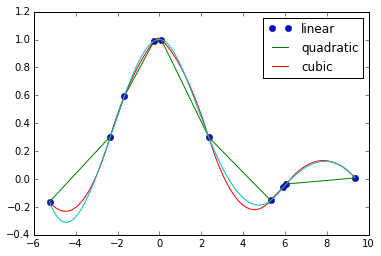
\includegraphics[height=5cm]{sinxx.png}
\end{figure}


\item La tercera interpolación es dados 20 puntos aleatorios entre x=-3 y x=3, para $f(x)=x^2 sin(2x)$.

\begin{verbatim}
import numpy as np
import matplotlib.pyplot as plt
from scipy.interpolate import interp1d


x0 = np.random.random(16)
x = (x0*6)-3
y = (x**2)*np.sin(2*x)


plt.plot(x, y, 'o', label='Data')


xp = np.linspace(min(x), max(x), 5100)
                
  
options = ('linear', 'quadratic', 'cubic')
for o in options:
    f = interp1d(x, y, kind=o)    
    plt.plot(xp, f(xp), label=o)    
    
plt.legend([ 'linear', 'quadratic', 'cubic'], loc='best')
plt.show()
\end{verbatim}
 Este código nos proporcionó la siguiente interpolación:
 \begin{figure}[H]
\centering
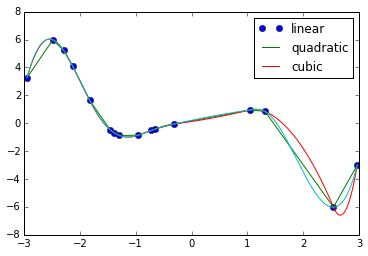
\includegraphics[height=5cm]{sinxxx.png}
\end{figure}


\item La cuarta interpolación es dados 12 puntos aleatorios entre x=-2 y x=2, para $f(x)=x^ sin(3x)$.

\begin{verbatim}
import numpy as np
import matplotlib.pyplot as plt
from scipy.interpolate import interp1d


x0 = np.random.random(12)
x = (x0*4)-2
y = (x**3)*np.sin(2*x)

plt.plot(x, y, 'o', label='Data')

xp = np.linspace(min(x), max(x), 5100)
                  
options = ('linear', 'quadratic', 'cubic')
for o in options:
    f = interp1d(x, y, kind=o)    
    plt.plot(xp, f(xp), label=o)    
    
plt.legend([ 'linear', 'quadratic', 'cubic'], loc='best')
plt.show()
\end{verbatim}
 Este código nos proporcionó la siguiente interpolación:
 \begin{figure}[H]
\centering
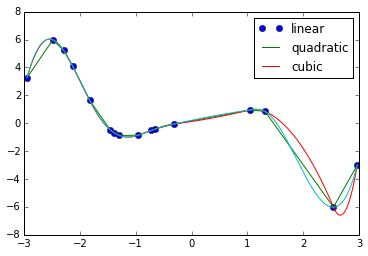
\includegraphics[height=5cm]{sinxxx.png}
\end{figure}

\end{enumerate}
\end{document}
